\section{Requirements and Design Consideration}

\noindent
The requirements for this project are clear and fixed. The functional requirements are as follows:
\begin{enumerate}
  \item The platform should scale easily with the number of devices and sensing parameters;
  \item WSN should be inexpensive and easy to deploy;
  \item The platform should have archival cloud storage with data analytics capability;
  \item The cloud service must be reliable and always on;
  \item Devices must be authenticated before sending telemetry data;
  \item Devices should be managed and reconfigured via over-the-air (OTA) updates;
  \item Data should be accessible in real-time by the user via MQTT; and
  \item The telemetry parameters required for each sensing node are given in Table~\ref{table:telemetryParameters}.
\end{enumerate}

\renewcommand{\floatpagefraction}{0.9}
\renewcommand{\arraystretch}{1.1}
\begin{table}[ht]
\centering
\begin{tabular}{ p{5.2cm} p{6.2cm}}
  \hline
  \textbf{Service Type} & \textbf{Telemetry Parameters}\\
  \hline
  Publish & Soil Temperature\\
  & Soil Moisture\\
  & Timestamp\\
  & NodeID\\
  & FarmID\\
  \hline
  Subscribe & Configuration State\\
  & Commands\\
  \hline
\end{tabular}
\caption{Device Telemetry Parameters} 
\label{table:telemetryParameters}
\end{table} 

\noindent
Based on the functional requirement, the proposed Software Design Considerations are given in Table~\ref{table:designConsideration}.

\renewcommand{\arraystretch}{1.2}
\begin{table}[ht]
\centering
\begin{tabular}{ p{0.4cm} p{5cm} p{6cm}}
  \hline
  & \textbf{Requirement} & \textbf{Design Consideration}\\
  \hline
  1 & Scalable with the number of devices and sensing parameters & An easily scalable WSN to be used.\\
  2 & WSN should be inexpensive and easy to deploy & WSN shouldn't be based on proprietary software/hardware; preferably consumer hardware\\
  3 & Cloud Platform must have archival cloud storage with data analytics capability & Utilizing Google BigQuery for its high throughput and big data analytics capability\\
  4 & Cloud service must be reliable and always on & Google Cloud Platform is reliable and has high availability\\
  5 & Devices must be authenticated before sending telemetry data & Sensing nodes will be authenticated using an intermediary device keeping the cost down\\
  6 & Devices should be managed and reconfigured via over-the-air (OTA) updates & GCP IoT Core provides device management and configuration over the air\\
  7 & Data should be accessible in real-time by the user via MQTT & Real-time data will be made available through an MQTT broker hosted by Google Cloud Pub/Sub\\
  \hline
\end{tabular}
\caption{Functional Requirements and Design Considerations} 
\label{table:designConsideration}
\end{table} 

\newpage
\section{Network Architecture}

The proposed network architecture (depicted in Figure~\ref{fig:layers}) is composed of 3 layers: sensor, gateway, and cloud back-end. In this section, we will discuss these three layers and their implementation.

\begin{figure}[!h]
  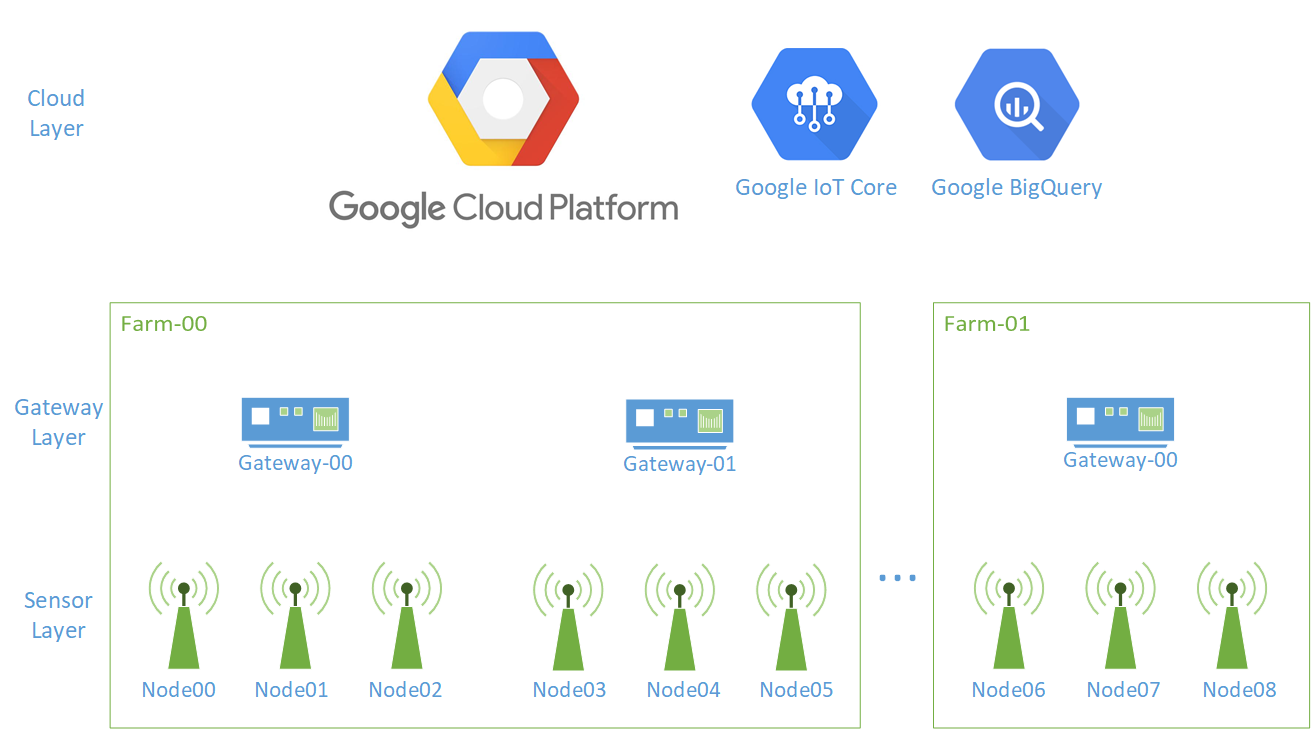
\includegraphics[width=\textwidth]{layers.png}
  \caption{Proposed 3-layer architecture}
  \label{fig:layers}
\end{figure}

\subsection{Sensor Layer}
  The sensor layer is comprised of the actual sensing hardware. Each device or node currently comprises of just 3 modules: an IoT capable micro-controller(ESP8266), the environmental sensors (Soil Moisture and Temperature), and a 3.2v battery (LiFePo4). The functionally modular design allows for easy upgradability and repair. The node design is given in Figure~\ref{fig:node}.
  
  \begin{figure}[!h]
    \centering
    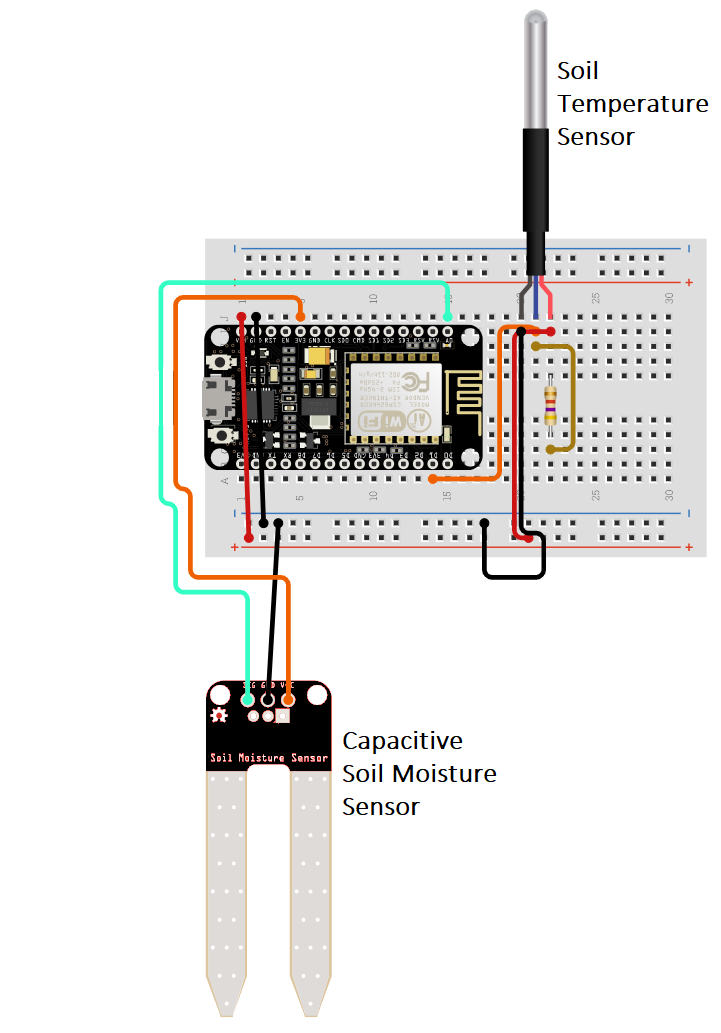
\includegraphics[width=0.7\textwidth]{node.png}
    \caption{Node Design Schematics}
    \label{fig:node}
  \end{figure}

  The ESP8266 microcontroller is a low-cost, low-power microcontroller with inbuilt WiFi capability and multiple GPIOs for communication purposes (Refer to Table~\ref{table:nodespecs}). The micro-controller is responsible for collecting the data from the sensors and sending it to the gateway through the mesh. The micro-controller is powered by a 3.3v power source and uses 80-90mA during load and 20\si{\micro\ampere} during deep sleep. Using a 1-3 hour duty cycle, the power consumption of the micro-controller can be reduced to less than 1mA per hour. Using a 3000mah battery, this can last anywhere from 150-215 days depending on external factors.
  
  \begin{table}[h]
    \centering
    \begin{tabular}{ p{5cm} p{5cm}}
      \hline
      \textbf{Parameters} & \textbf{Specification}\\
      \hline
      Processor & TenSilica L106 80MHz 32bit\\
      SRAM & 160 kbytes\\
      Flash Storage & SPI Flash, up to 16 MBytes\\
      GPIO pins & 17\\
      ADC pins & 1 pin, 10 bit\\
      WiFi & 2.4GHz, 802.11 b/g/n\\
      Operating Voltage & 3-3.6 Volts\\
      \hline
    \end{tabular}
    \caption{ESP8266 (Sensor Node) Specifications} 
    \label{table:nodespecs}
  \end{table}

  \FloatBarrier
  \begin{table}[h]
    \centering
    \begin{tabular}{ p{5cm} p{5cm}}
      \hline
      \textbf{Sensor} & \textbf{Model}\\
      \hline
      Soil Temperature & DS18B20\\
      Soil Moisture (Capacitive) & RKI-3225\\
      \hline
    \end{tabular}
    \caption{Used Sensor Models} 
    \label{table:sensors}
  \end{table}

\subsection{Gateway Layer}

  The gateway layer comprises aggregating devices that connect to WSN networks, collect the data, authenticate the devices, and then relay the data to the cloud. During each duty cycle, the gateway will wake up and perform the following:
  \begin{enumerate}
    \item Connect to the WSN using wifi;
    \item Authenticate active sensor nodes using a JSON Web Token (JWT);
    \item Collect sensor reading and calculate any derived measurements;
    \item Relay to Cloud MQTT broker and the BigQuery database for archival storage with proper timestamps; and
    \item Receive any configuration updates and relay them to the respective node in the WSN.
  \end{enumerate}
  The gateway is implemented using Raspberry Pi 4 (4GB) micro-controller. Being equipped with a 1.5GHz quad-core CPU and 4 GB RAM, it is more than capable enough to handle multiple data streams and adds to the scalability of the design. These devices provide sufficient edge processing, removing any requirement for cloud-based processing power. The inbuilt WiFi(2.4 GHz and 5.0 GHz), Bluetooth 5.0, and BLE modules can be used for connecting to both Wifi and BLE based WSNs. A 4G USB dongle is used to provide internet connectivity in remote areas, but an ethernet interface can also be used for the same.

  \FloatBarrier
\subsection{Cloud Layer}
  The cloud layer is responsible for data ingestion, device management through the gateway, and providing archival storage and data analytics. The cloud architecture is described in Figure~\ref{fig:cloud}.


  \begin{figure}[!h]
    \centering
    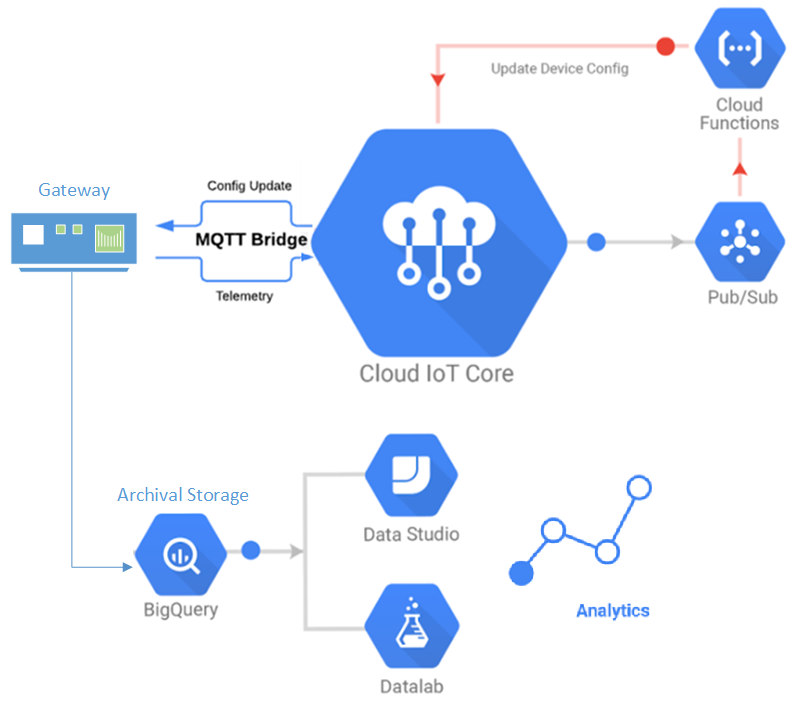
\includegraphics[width=0.9\textwidth]{cloud.png}
    \caption{GCP Cloud Architecture}
    \label{fig:cloud}
  \end{figure}  

  The Google Cloud Platform (GCP) is used for the same as Google Cloud IoT core platform has the functionality to support data ingestion from a large number of globally distributed devices. The platform also has integrated services that manage authentication and device management. Google BigQuery is used for archival storage and data analytics as it supports direct streams of data and has high throughput \cite{iotCore,ref1.13}. 
  
  A direct connection between an ESP8266-based node and Google Cloud IoT Core is possible but since many inexpensive boards lack the features required to make a secure connection, the WSN is kept isolated. The gateway layer handles the authentication process for the nodes through JSON Web Token (JWT) authentication. Each node must be authenticated via the gateway it is bound to before it can send any telemetry data.
